\section{Moving} \label{moving}
A character's movement is defined by their Agility score.
By default, a character can move $Agi / 2$ number of hexes (rounded down).
So if the character has an agility of 13, they can move at most 6 hexes in a single turn.
That this can change if a character's special ability says otherwise.

\begin{note}
    You \textit{\textbf{cannot}} go back to a character you have already moved.
\end{note}

\subsection{Tackle Zones \& Opportunity Attacks}
Every character has a tackle zone around them (see Figure~\ref{fig:tackle-zone-1}).
The tackle zone is made up of every hex immediately around a character.

If an opponent \textit{leaves} a hex within the tackle zone of your character, they must first roll against their agility score to see if they successfully dodge your attack.
If they fail, you get to attack them as normal (see \textit{Attacking} in Section \ref{attacking}).
If they succeed, they get to move as usual.

\paragraph{Note} Tackle zones can also overlap (see figure \ref{fig:tackle-zone-2}).
If your character tries to move out of an overlapping tackle zone, only roll for the one you're actually leaving.
If you're leaving both at once, you must escape the one with the highest Agility first.
Failing one fails them both.

\begin{figure}
    \centering
    
\includegraphics{graphics/tackle-zones-1.png}
    \caption{The tackle zone around a character.}
    \label{fig:tackle-zone-1}
\end{figure}

\begin{figure}
    \centering
    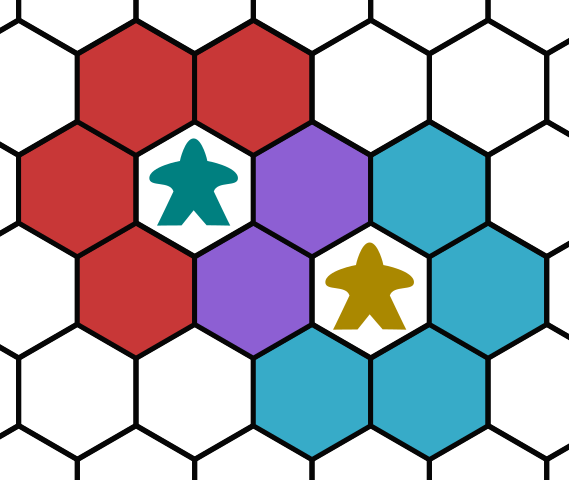
\includegraphics{graphics/tackle-zones-2.png}
    \caption{The overlapping tackle zones between two characters.}
    \label{fig:tackle-zone-2}
\end{figure}